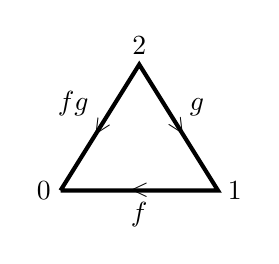
\begin{tikzpicture}
\node[above] (c) at (1,1.6) {$2$};
\node[left]  (a) at (0,0) {$0$};
\node[right] (b) at (2,0) {$1$};
\draw[line width=1.5px] (0,0) 
    -- (2,0)    node[sloped, scale=.9, pos=0.5] {$<$} 
                node[scale=1, pos=0.5, below] {$f$} 
    -- (1,1.6)  node[sloped, scale=.9, pos=0.5] {$>$} 
                node[scale=1, pos=0.5, above right] {$g$}
    -- (0,0)    node[sloped, scale=.9, pos=0.5] {$<$} 
                node[scale=1, pos=0.5, above left] {$fg$};
\end{tikzpicture}